\documentclass{article}
\usepackage[T1]{fontenc}
\usepackage{lmodern}
\usepackage{graphicx}
\usepackage{amsmath,amssymb}
\usepackage[a4paper,margin=2cm]{geometry}
\usepackage[absolute,overlay]{textpos}
\setlength{\TPHorizModule}{1mm}
\setlength{\TPVertModule}{1mm}
\usepackage[indonesian]{babel}
\usepackage{hyperref}
\setlength{\emergencystretch}{2em}
% unit: Halaman 19

\begin{document}

% === Halaman 19 (llm) ===

\begin{center}
\textbf{Teknik Steganalisis: Visual Attack}
\end{center}

\vspace{10mm}

\begin{center}
\begin{tabular}{cccc}
Gambar asli & Hasil penapisan (asli) & Terdeteksi ada pesan & Terdeteksi ada pesan
\end{tabular}
\end{center}

\vspace{10mm}

\begin{center}
\begin{tabular}{cc}
Terdeteksi ada pesan & Terdeteksi ada pesan
\end{tabular}
\end{center}

% deskripsi: Kumpulan gambar contoh visual attack pada steganografi, menampilkan gambar asli kincir angin, hasil penapisan, dan beberapa variasi deteksi pesan dengan artefak visual berupa noise warna-warni.
% bbox normalisasi: [0.1600, 0.2300, 0.8800, 0.5500]
\begin{textblock*}{151.20mm}(33.60mm,68.31mm)
\noindent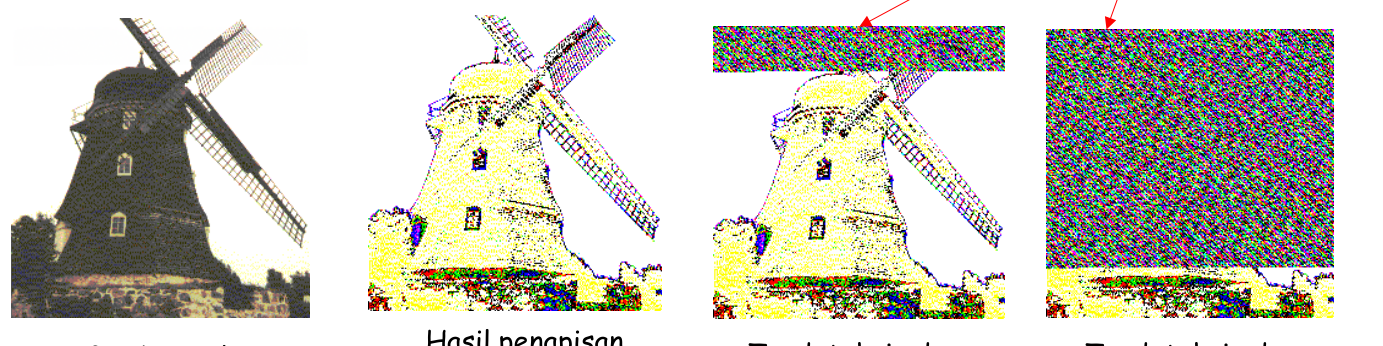
\includegraphics[width=151.20mm,height=95.04mm]{../../images/llm/page_019_img_01.png}%
\end{textblock*}

% deskripsi: Dua contoh gambar tambahan yang menunjukkan deteksi adanya pesan melalui analisis visual dengan noise warna-warni.
% bbox normalisasi: [0.2400, 0.6300, 0.6900, 0.9100]
\begin{textblock*}{94.50mm}(50.40mm,187.11mm)
\noindent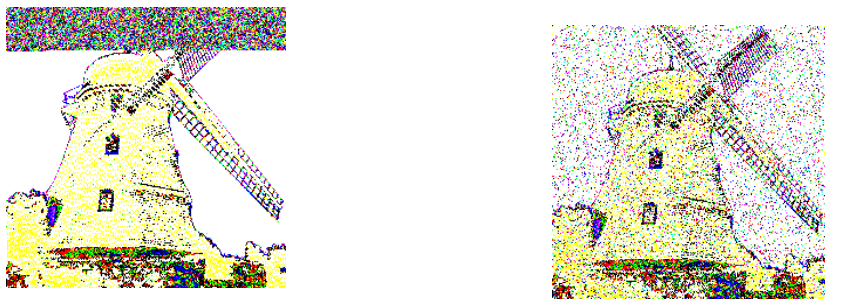
\includegraphics[width=94.50mm,height=83.16mm]{../../images/llm/page_019_img_02.png}%
\end{textblock*}

\end{document}
